\chapter{Durchführung}
\label{chap:Durchfuehrung}

In diesem Kapitel wird die Durchführung der Parameterstudie erläutert. Zuerst werden neue Gleichungen in das Skript eingearbeitet. Dann wird das Vorgehen vorgestellt und die Auswertungskriterien und Annahmen festgelegt.\\
Für die Parameterstudie werden die Höhe, die Geschwindigkeit, der Kugelradius, die Auftreffstelle und das Seitenverhältnis variiert.

In der bereits hergeleiteten Theorie wird der Lösungsweg für den Stoßvorgang vorgestellt. Mit dem zur Verfügung gestellten Skript, das auf dieser Theorie basiert, wird nun die Para-meterstudie durchgeführt. Um relevante Ergebnisse zu erlangen, müssen zuerst weitere Gleichungen in das Skript eingearbeitet werden.\\
In dem Skript wird eine Konstante $c$ als Vorfaktor für die Kraftberechnung aus dem Punkt-kontakt verwendet. Um die Berechnungsmöglichkeiten zu erweitern, wird $c$ nun durch eine Gleichung der Hertz'schen Pressung ersetzt, die wie folgt hergeleitet wird:\\

Die Gleichung für die Hertz'sche Pressung eines Kugel-Kugel-Punktkontaktes lautet wie in Gleichung~\ref{form:ZvonP}.

\begin{equation}
	\label{form:ZvonP}
	z(P) = \left[ \frac{9 P^{2} (1 - \nu^{2})^{2}}{2 E^{2}} \cdot \left( \frac{1}{2 r_{1}} + \frac{1}{2 r_{2}} \right) \right]^{\frac{1}{3}}
\end{equation}

Hier ist wieder "g" kurz für Gewicht nach Karas~\cite{Karas.1939}. Da einer der beiden Körper eine Platte mit dem Radius $r_{p} = \infty$ ist, folgt durch Einsetzen von $r_{p}$ und Umstellen nach P:

\begin{equation}
	\label{form:PvonZ}
	P(z) = \sqrt{\frac{4 r_{g}}{9}} \cdot \frac{E}{(1 - \nu^{2})} \cdot z^{\frac{3}{2}}
\end{equation}
	
Hier ist $\frac{E}{(1 - \nu^{2})}$ der reduzierte E-Modul, welcher durch Gleichung~\ref{form:redE} beschrieben wird.

\begin{equation}
	\label{form:redE}
	\frac{E}{(1 - \nu^{2})} = 2 \cdot \left( \frac{(1 - \nu_{p}^{2})}{E_{p}} + \frac{(1 - \nu_{g}^{2})}{E_{g}} \right)^{-1}
\end{equation} 

Nun wird $c$ als Vorfaktor von $z^{\frac{3}{2}}$ in Gleichung~\ref{form:PvonZ} definiert, so dass folgt:

\begin{equation}
	\label{form:c}
	c = \sqrt{\frac{4 r_{g}}{9}} \cdot \frac{E}{(1 - \nu^{2})}
\end{equation}

Im Skript wurden Gleichungen~\ref{form:redE} und~\ref{form:c} unter den Konstanten implementiert und die einstellbaren Parameter der Platte und der Impaktor respektive um $E_{p}$ und $\nu_{p}$, bzw. $E_{g}$ und $\nu_{g}$ erweitert.\\

\section{Vorgehen und Vorbereitung}

Insgesamt wird der Stoßvorgang durch die einstellbaren Parameter in Tabelle~\ref{tab:VariablenderStudie} beschrieben. In Anlehnung an \cite{Olsson.2000} wird das Massenverhältnis $MR$ als einer der signifikanten Parameter gewählt. Davon ausgehend werden dann die anderen Parameter individuell variiert und die Ergebnisse grafisch ausgewertet. 

\begin{table}[H]
	\begin{center}
		\caption{Variablen der Parameterstudie}
		\label{tab:VariablenderStudie}
		\begin{tabular}{l|c}
			\textbf{Variable} & \textbf{Bedeutung}\\
			\hline
			$a,b,h$ & Plattenmaße in [cm]\\
			$r_{g}$ & Impaktorradius in [cm]\\
			$v_{0}$ & Auftreffgeschwindigkeit [cm/s]\\
			5 & Massenverhältnis $\hat{=}$ $\frac{Impaktormasse}{Plattenmasse}$\\
			$\xi,\eta$ & Auftreffstelle des Impaktors\\
			$x,y$ & Auswertungsstelle\\		
		\end{tabular}
	\end{center}
\end{table}

\subsection*{Auswertungskriterien und Annahmen}

Als Auswertungskriterien werden die Anzahl der einzelnen Schläge, die maximal auftretenden Kraft und die Auslenkung der Platte gewählt. \\
Für die Studie werden folgende übergreifende Annahmen getroffen: 

\begin{enumerate}
	\item{Die Platte und der Impaktor sind isotrop mit konstanten Stoffwerten.}
	\item{Die Platte und der Impaktor sind aus identischem Material, mit gleichem E-Modul und Poissonzahl $\nu$.}
\end{enumerate}

\newpage
\subsubsection*{Anzahl der Schläge}

Als Schlag wird hier ein Kraftverlauf bezeichnet, bei dem die Kraft $P_{i}$ zwischen den Schlägen auf Null fällt, nach der Bedingung in Gleichung~\ref{form:Schlagauftreten}:

\begin{equation} 
	\label{form:Schlagauftreten}
	F_{i-1} > 0 \; \wedge \; F_{i} = 0.0 
\end{equation}

Die Schrittanzahl $i$ wird hier durch empirische Beobachtungen festgelegt. Zuerst wurde überprüft, ab wann der Stoßvorgang sich periodisch wiederholt. Ab $i = 500$ bilden sich bei einer signifikanten Anzahl von Parametervariationen periodische Wiederholungen aus. Um sicherzustellen, dass die Ergebnisse nicht verfälscht werden, wurde nun $i = 1000$ gesetzt.\\
Da $\tau$ aus Gleichung~\ref{eq:tau} von den geometrischen Parametern der Platte abhängt, wird $\tau$ bei jeder Geometrieänderung neu berechnet.


\subsubsection*{Maximale Auslenkung der Platte}

Die maximale Auslenkung $w_{max}$ wird direkt aus der Versuchsreihe ausgelesen und in Abhängigkeit des Massenverhältnisses und des zu verändernden Parameters dargestellt.

\subsubsection*{Maximale Kraft}

Analog zur maximalen Auslenkung, wird die maximale Kraft $P_{max}$ direkt ausgelesen und in Abhängigkeit von $MR$ und dem Parameter dargestellt.

\newpage

\section{Parameterstudie}

Für die Parameterstudie wurde folgender Fall als Ausgangspunkt gewählt: 

\begin{table}[H]
	\begin{center}
		\caption{Ausgangsfall Parameterstudie}
		\label{tab:Ausgang}
		\begin{tabular}{l|c}
			\textbf{Variable} & \textbf{Wert}\\
			\hline
			$a$ & 50.0 [cm]\\
			$b$ & 50.0 [cm]\\
			$h$ & 1.0 [cm]\\
			$r_{g}$ & 1.0 [cm]\\
			$v_{0}$ & 440.0 [cm/s]\\
			$\xi,\eta$ & 25.0 [cm]\\
			$x,y$ & 25.0 [cm]\\ 		
		\end{tabular}
	\end{center}
\end{table}

Der Radius muss gesondert erwähnt werden, da er für die Studie konstant gehalten wird. Wenn die Impaktormasse bei konstantem Radius erhöht wird, ändert sich die Geometrie nach Abbildung~\ref{fig:konstRad}. Dadurch ergibt sich bei kleinen Massenverhältnissen ein schalenförmiger Impaktkörper. Die Berechnung kann numerisch bei solchen $MR$ durchgeführt werden, ergibt jedoch physikalisch nur bedingt Sinn. Für die Kontinuität wurden diese $MR$ in der Studie berücksichtigt, es besteht jedoch Bedarf für weitere Recherche in diesem Bereich. 

\begin{figure}[H]
	\begin{center}
		\begin{overpic}[width=\linewidth]{pictures/durchfuehrung/Radius.eps}
			\put(57,23){$r_{g}$}
			\put(47,2){Platte}
			\put(48,19){$m_{g,i}$}
			\put(47,29.7){$\Delta m_{g,i+1}$}
			\put(47,39.6){$\Delta m_{g,i+2}$}
		\end{overpic}
	\caption{Impaktormassenänderung bei konstantem Radius}
	\label{fig:konstRad}	
	\end{center}
\end{figure}

$MR$ wird in Tabelle~\ref{tab:Ausgang} bewusst ausgelassen, da bei jedem Parameter außer der Auftreffstelle über das Massenverhältnis iteriert wird und dadurch kein Anfangswert, sondern eine Menge benötigt wird. Die Menge der $MR$ ist nach Gleichung~\ref{form:MR}:

\begin{equation}
	\label{form:MR}
	0.1 \leq MR \leq 2.50 \; , \;\; \mbox{Schrittweite:} \; \Delta MR = 0.01
\end{equation}

Die Stoffparameter bleiben konstant und entsprechen in Tabelle~\ref{tab:Stoff} den Werten von Stahl.

\begin{table}[H]
	\begin{center}
		\caption{Stoffparameter: Kugel und Platte}
		\label{tab:Stoff}
		\begin{tabular}{l|c}
			\textbf{Variable} & \textbf{Wert}\\
			\hline
			$E_{p}$ & $2.2 \cdot 1e06$ [$kg/cm^2$]\\
			$\nu_{p}$ & 0.3 [-]\\
			$\rho_{p}$ & 0.00796 [$kg/cm^{3}$]\\
			\hline
			$E_{g}$ &  $2.2 \cdot 1e06$ [$kg/cm^2$]\\
			$\nu_{g}$ & 0.3 [-]\\		
		\end{tabular}
	\end{center}
\end{table}

\subsection{Höhe der Platte}

Als erster Parameter wird die Höhe nach Gleichung~\ref{form:DeltaH} variiert. Alle anderen Werte werden nach Tabelle~\ref{tab:Ausgang} konstant gehalten.

\begin{equation}
	\label{form:DeltaH}
	0.5 cm \leq h \leq 2.5 cm, \; \; \mbox{Schrittweite:} \; \Delta h = 0.02 cm
\end{equation}

Wenn man die Höhe, das Massenverhältnis und die Anzahl der Schläge aufträgt, ergibt sich Abbildung~\ref{fig:Hoehe}.\\
Man kann direkt ablesen, dass mehrere Aufschläge vermehrt im unteren Höhenbereich auftreten. Dies ist auf die Steifigkeit der Platte zurückzuführen. Bei größerer Plattendicke ist die Platte steifer und die Kugel prallt ab, ohne häufiger aufzutreffen. Bei $h = 0.6 cm$ treten bis zu 10 Schläge auf.\\
Es ist offensichtlich, dass bei einem Massenverhältnis $MR \geq 1.7$ und einer Plattendicke von $h \geq 1.6 cm$ nur noch einzelne Stöße auftreten. Hier ist anzunehmen, dass der elastische Stoßvorgang der Kugel ausreichend kinetische Energie entgegen der Stoßrichtung überträgt, sodass die Kugel sich schneller entfernt als die Platte auslenken kann. \\

\begin{figure}[H]
	\begin{center}
		\begin{overpic}[scale=1]{pictures/gnuplot/3d/Hoehe/production/Hoehe.eps}
			\put(40,-1.5){Höhe [cm]}
			\put(7,33){\rotatebox{90}{MR [-]}}
			\put(83,70){Aufschläge [-]}
		\end{overpic}
		\caption{Höhe, MR und Anzahl der Aufschläge}
		\label{fig:Hoehe}
	\end{center}
\end{figure}

Auch bei der Auslenkung stimmen die Ergebnisse mit den Erwartungen überein. In Abbildung~\ref{fig:HoeheAuslenkung} ist zu erkennen, dass mit zunehmender Höhe die Auslenkung abfällt, da die Steifigkeit der Platte zunimmt. Die Steigung der Auslenkungskurve flacht mit zunehmendem $MR$ ab. Am größten ist die Steigung im Bereich $0.1 \leq MR \leq 1$. Daher ist der Einfluss des Massenverhältnisses in diesem Bereich am signifkantesten.\\
Bei Plattendicken von $h \geq 1.3 cm$ flacht die Steigung der maximalen Auslenkung in einen annähernd linearen Bereich ab. Daher liegt nahe, dass die Höhe im Bereich bis $h = 1.3 cm$ den stärksten Einfluss hat.\\
In Tabelle~\ref{tab:WKHoehe} sind die minimalen und maximalen Werte der Auslenkung und Kraft sowie die Faktoren, die zwischen diesen Werten liegen, aufgeführt.
Wenn man die maximal auftretende Kraft betrachtet, ergibt sich Abbildung~\ref{fig:HoeheKraft}.\\
Aus der maximalen Auslenkung kann man für die Höhe schlussfolgern, dass die maximale Kraft dort auftritt, wo die Auslenkung am geringsten ist, da hier am wenigsten Energie in die Deformation der Platte übergeht.\\

\begin{table}[H]
	\begin{center}
		\caption{Auslenkung und Kraft}
		\label{tab:WKHoehe}
		\begin{tabular}{l|c|c|r}
			\textbf{Auslenkung/Kraft} & \textbf{Höhe [cm]} & \textbf{MR} & \textbf{Wert}\\
			\hline
			$w_{max}$ & 0.64  & 2.42 & 2.112 cm\\
			$w_{min}$ & 2.5  & 0.1 & 0.0846 cm\\
			\hline
			$P_{max}$ & 2.5  & 2.5 & 619.77 kN\\
			$P_{min}$ & 0.64  & 0.1 & 158.62 kN\\
			\hline
			Faktor : $\frac{w(MR_{max})}{w(MR_{min})}$ & $h_{min}=0.5$ & & 4.72\\
			Faktor : $\frac{w(MR_{max})}{w(MR_{min})}$ & $h_{max}=2.5$ & & 5.33\\
			\hline
			Faktor : $\frac{P(MR_{max})}{P(MR_{min})}$ & $h_{min}=0.5$ & & 0.98\\
			Faktor : $\frac{P(MR_{max})}{P(MR_{min})}$ & $h_{max}=2.5$ & & 4.96\\
		\end{tabular}
	\end{center}
\end{table}

\begin{figure}[h!]
	\begin{center}
		\begin{overpic}[width=\linewidth]{pictures/gnuplot/3d/Hoehe/production/HoeheAuslenkung3D.eps}
			\put(22,8){Höhe [cm]}
			\put(75,12){MR [-]}
			\put(83,55){Auslenkung [cm]}
		\end{overpic}
	\caption{Auslenkung in Abhängigkeit der Höhe und MR}
	\label{fig:HoeheAuslenkung}
	\end{center}
\end{figure}

\begin{figure}[H]
	\begin{center}
		\begin{overpic}[width=\linewidth]{pictures/gnuplot/3d/Hoehe/production/HoeheKraft3D.eps}
			\put(22,8){Höhe[cm]}
			\put(75,12){MR [-]}
			\put(87,55){Kraft [N]}
		\end{overpic}
	\caption{Kraft in Abhängigkeit der Höhe und MR}
	\label{fig:HoeheKraft}
	\end{center}
\end{figure}

\newpage

\subsection{Geschwindigkeit des Impaktors}

Als nächster Parameter wird die Geschwindigkeit betrachtet. Da hier nur der Low-Velocity Bereich betrachtet wird, wird die Geschwindigkeit nach Gleichung~\ref{form:DeltaV0} variiert. 

\begin{equation}
	100 cm/s \leq v_{0} \leq 1000 cm/s \; , \;\; \mbox{Schrittweite:} \; \Delta v_{0} = 10 cm/s
	\label{form:DeltaV0}
\end{equation}

Analog zur Höhenvariation wird zunächst die Anzahl der Aufschläge aufgetragen. In Abbildung~\ref{fig:Speed} ist zu erkennen, dass die Geschwindigkeit bei gleichbleibendem $MR$ nur einen verschwindend geringen Einfluss auf die Anzahl der Aufschläge hat. 

\begin{figure}[h!]
	\begin{center}
		\begin{overpic}[scale=1]{pictures/gnuplot/3d/Speed/production/Speed.eps}
			\put(35,-1.5){Geschwindigkeit [cm/s]}
			\put(7,33){\rotatebox{90}{MR [-]}}
			\put(83,70){Aufschläge [-]}
		\end{overpic}
		\caption{Geschwindigkeit, MR und Anzahl der Aufschläge}
		\label{fig:Speed}
	\end{center}
\end{figure}

Die aus den Stößen resultierende Auslenkung wird in Abbildung~\ref{fig:SpeedAuslenkung} dargestellt. Man kann erkennen, dass der Einfluss des Massenverhältnisses mit steigender Geschwindigkeit zunimmt. \\
Auch deutlich ist, dass im höheren Geschwindigkeitsbereich die Auslenkung stärker mit größer werdendem $MR$ ansteigt. \\
Zuletzt wird die Kraft aufgetragen. In Abbildung~\ref{fig:SpeedKraft} sind ähnliche Trends wie in Abbildung~\ref{fig:SpeedAuslenkung} zu sehen. \\
Auch hier nimmt die auftretende Kraft mit $v_{0}$ zu.  Je größer $MR$ hierbei ist, desto steiler die Kraftzunahme.\\
Analog zur Höhe werden hier auch die Werte in Tabelle~\ref{tab:WKSpeed} dargestellt. 

\begin{table}[H]
	\begin{center}
		\caption{Auslenkung und Kraft}
		\label{tab:WKSpeed}
		\begin{tabular}{l|c|c|r}
			\textbf{Auslenkung/Kraft} & \textbf{Geschwindigkeit [cm/s]} & \textbf{MR} & \textbf{Wert}\\
			\hline
			$w_{max}$ & 1000  & 2.5 & 2.58 cm\\
			$w_{min}$ & 100  & 0.1 & 0.046 cm\\
			\hline
			$P_{max}$ & 1000  & 2.5 & 318.58 kN\\
			$P_{min}$ & 100 & 0.1 & 7.094 kN\\
			\hline
			Faktor : $\frac{w(MR_{max})}{w(MR_{min})}$ & $v_{0,min}=100 $ & & 5.55\\
			Faktor : $\frac{w(MR_{max})}{w(MR_{min})}$ & $v_{0,max}=1000 $ & & 5.77\\
			\hline
			Faktor : $\frac{P(MR_{max})}{P(MR_{min})}$ & $v_{0,min}=100$ & & 3.90\\
			Faktor : $\frac{P(MR_{max})}{P(MR_{min})}$ & $v_{0,max}=1000$ & & 3.92\\
		\end{tabular}
	\end{center}
\end{table}

\begin{figure}[H]
	\begin{center}
		\begin{overpic}[width=\linewidth]{pictures/gnuplot/3d/Speed/production/SpeedAuslenkung3D.eps}
			\put(62,9.5){Geschwindigkeit [cm/s]}
			\put(14,12){MR [-]}
			\put(83,55){Auslenkung [cm]}
		\end{overpic}
		\caption{Auslenkung in Abhängigkeit der Geschwindigkeit und MR}
		\label{fig:SpeedAuslenkung}
	\end{center}
\end{figure}

\begin{figure}[H]
	\begin{center}
		\begin{overpic}[width=\linewidth]{pictures/gnuplot/3d/Speed/production/SpeedKraft3D.eps}
			\put(62,9.5){Geschwindigkeit [cm/s]}
			\put(14,12){MR [-]}
			\put(85,55){Kraft [N]}
		\end{overpic}
		\caption{Kraft in Abhängigkeit der Geschwindigkeit und MR}
		\label{fig:SpeedKraft}
	\end{center}
\end{figure}

\newpage

\subsection{Impaktorradius}

Im Folgenden wird der Radius des Impaktors betrachtet. Nach Gleichung~\ref{form:Radius} wird der Radius der Kugel erhöht.

\begin{equation}
	0.5 cm\leq r_{g} \leq 10 cm, \; \; \mbox{Schrittweite:} \; \Delta r_{g} = 0.1 cm
	\label{form:Radius}
\end{equation}

In Abbildung~\ref{fig:Radius} ist zu erkennen, dass der Radius nur einen geringen Einfluss auf die Anzahl der Aufschläge hat.\\
Bildet man die Daten in 3D ab, erkennt man leicht, dass die Anzahl der Aufschläge sich signifikant nur mit $MR$ verändert. \\

\begin{figure}[H]
	\begin{center}
		\begin{overpic}[scale=1]{pictures/gnuplot/3d/Radius/production/Radius.eps}
			\put(37,-1.5){Radius [cm]}
			\put(7,33){\rotatebox{90}{MR [-]}}
			\put(83,70){Aufschläge [-]}
		\end{overpic}
		\caption{Radius, MR und Anzahl der Aufschläge}
		\label{fig:Radius}
	\end{center}
\end{figure}

Ähnliche Ergebnisse werden auch bei der Auslenkung erreicht. Wie in Abbildung~\ref{fig:RadiusAuslenkung} zu sehen ist, nimmt die Auslenkung nur bei hohen $MR$ auch durch Erhöhung des Radius zu.\\
In Tabelle~\ref{tab:WKSpeed} sind die maximalen und minimalen Werte aufgetragen.\\
Im niederen $MR$-Bereich sind die Auslenkungen bei $r_{g} = 0.5 cm$ und bei $r_{g} = 10.0 cm$ fast identisch.  Bei $MR_{max} = 2.5$ ist die Auslenkung jedoch nur auf der zweiten Nachkommastelle größer.\\
Auch wenn man die Kraft betrachtet, lassen sich ähnliche Trends erkennen. In Abbildung~\ref{fig:RadiusKraft} verändert sich die resultierende maximale Kraft im niederen $MR$-Bereich nur minimal.\\
Analog zu der Auslenkung ergibt sich die signifikanteste Kraftänderung bei $MR_{max}$. 

\begin{table}[H]
	\begin{center}
		\caption{Auslenkung und Kraft}
		\label{tab:WKRadius}
		\begin{tabular}{l|c|c|r}
			\textbf{Auslenkung/Kraft} & \textbf{Radius [cm]} & \textbf{MR} & \textbf{Wert}\\
			\hline
			$w_{max}$ & 10 & 2.5 & 1.14 cm\\
			$w_{min}$ & 0.5 & 0.01 & 0.201 cm\\
			\hline
			$P_{max}$ & 10 & 2.5 & 162.953 kN\\
			$P_{min}$ & 0.5 & 0.01 & 32.788 kN\\
			\hline
			Faktor : $\frac{w(MR_{max})}{w(MR_{min})}$ & $r_{min}=0.5 cm$ & & 5.63\\
			Faktor : $\frac{w(MR_{max})}{w(MR_{min})}$ & $r_{max}=10 cm$ & & 5.86\\
			\hline
			Faktor : $\frac{P(MR_{max})}{P(MR_{min})}$ & $r_{min}=0.5 cm$ & & 3.78\\
			Faktor : $\frac{P(MR_{max})}{P(MR_{min})}$ & $r_{max}=10 cm$ & & 4.20\\
		\end{tabular}
	\end{center}
\end{table}

\begin{figure}[H]
	\begin{center}
		\begin{overpic}[scale=1]{pictures/gnuplot/3d/Radius/production/RadiusAuslenkung3D.eps}
			\put(62,9.5){Radius [cm]}
			\put(14,12){MR [-]}
			\put(83,55){Auslenkung [cm]}
		\end{overpic}
		\caption{Auslenkung in Abhängigkeit des Radius und MR}
		\label{fig:RadiusAuslenkung}
	\end{center}
\end{figure}

\begin{figure}[H]
	\begin{center}
		\begin{overpic}[scale=1]{pictures/gnuplot/3d/Radius/production/RadiusKraft3D.eps}
			\put(62,9.5){Radius [cm]}
			\put(14,12){MR [-]}
			\put(85,55){Kraft [N]}
		\end{overpic}
		\caption{Kraft in Abhängigkeit des Radius und MR}
		\label{fig:RadiusKraft}
	\end{center}
\end{figure}

\newpage

\subsection{Variation des Impaktortes}
Im Folgenden wird der Aufschlagsort des Impaktors verändert. Alle anderen Parameter aus Tabelle \ref{tab:Ausgang} und \ref{tab:Stoff} werden konstant gehalten. Um eine allgemeine Aussage zu ermöglichen, wurde der Aufschlagsort entdimensioniert. Hierfür werden $\xi$ und $\eta$ durch $a$, bzw. $b$ geteilt. Man erhält $\frac{\xi}{a}$ und $\frac{\eta}{b}$. Da die Durchführung für eine quadratische Platte gemacht wurde, musste aufgrund der Symmetrie lediglich ein Achtel der gesamten Platte berechnet werden mit:

$$\left\lbrace  \left(\frac{\xi}{a},  \frac{\eta}{b}\right) \in \mathbb{R}^2 \vert \ 0.5 \le \frac{\xi}{a} \le 1 \ \land \ 0.5 \le \frac{\eta}{b} \le \frac{\xi}{a}  \right\rbrace $$


\begin{figure}[H]
	\begin{center}
		\begin{overpic}[width=\linewidth]{pictures/gnuplot/3d/xieta/production/XiEta.eps}
			\put(50,3){$\frac{\xi}{a}$ [-]}
			\put(78,62){Aufschläge [-]}
			\put(15,35){$\frac{\eta}{b}$ [-]}
		\end{overpic}
		\caption{Anzahl der Schläge in Abhängigkeit des Auftreffpunktes}
		\label{fig:xiEta}
	\end{center}
\end{figure}


Zunächst wird  der Einfluss der Position des Aufschlags auf die Anzahl der Schläge zwischen Platte und Kugel in Abbildung~\ref{fig:xiEta} untersucht. Da ein Versuch mit einem Massenverhältnis von $1$ zu sehr überzogenen Werten geführt hat, welche im Rahmen der linearen Berechnungen keine Sinn ergibt, wurde die zeitliche Schrittweite vergrößert und das Massenverhältnis auf $0.3$ reduziert. Jedoch sind die Ergebnisse qualitativ gleich.	
Es ist klar zu erkennen, dass ab einem gewissen Radius die Anzahl der Aufschläge konstant bei eins liegt. Dieser Radius liegt im Fall der quadratischen Platte unter den gegebenen Parametern bei ca. $0.2 \cdot a$. Da die Anzahl der Aufschläge in der Regel eine gewisse Abhängigkeit mit der Steifigkeit der Platte aufweist, ist ersichtlich, dass die Platte am Rand eine erhöhte Steifigkeit aufweist und somit weniger Aufschläge hier stattfinden.\\
Interessant ist jedoch das kreisförmige Ausbreiten der Grenze zwischen einem und zwei Aufschlägen. Ebenfalls ist die Unregelmäßigkeit der Anzahl der Aufschläge innerhalb dieses Kreises auffällig. Wenn die Plattensteifigkeit gering genug ist, kann beobachtet werden, dass der erste Aufschlag teilweise die Geschwindigkeit der Kugel nur gering beeinflusst und durch eine höhere Relativgeschwindigkeit zwischen Platte und Kugel eine erhöhte Kraft beim zweiten Aufschlag beobachtet werden kann.

\begin{figure}[H]
	\begin{center}
		\begin{overpic}[width=\linewidth]{pictures/gnuplot/3d/xieta/production/XiEtaAuslenkung.eps}
			\put(50,3){$\frac{\xi}{a}$ [-]}
			\put(78,62){Auslenkung [cm]}
			\put(15,35){$\frac{\eta}{b}$ [-]}
		\end{overpic}
		\caption{Maximale Durchbiegung in Abhängigkeit des Auftreffpunktes}
		\label{fig:xiEtaAuslenkung}
	\end{center}
\end{figure}


Im Allgemeinen ist in den Abbildungen~\ref{fig:xiEtaAuslenkung} und ~\ref{fig:xiEtaKraft} ein Zusammenhang zwischen maximaler Durchbiegung und maximaler Kraft festzustellen.
Dieser Zusammenhang gilt jedoch nicht in Randnähe, da aufgrund der gegebenen Randbedingungen ein Absinken der Platte am Rand stark behindert ist.\\
Für die maximale Durchbiegung in Abhängigkeit des Aufschlagortes ergibt sich ein ähnliches Ergebnis wie für die Anzahl der Aufschläge. Zunächst ist ebenfalls eine klare, kreisförmige Grenze ersichtlich, mit dem gleichen Radius wie in \ref{fig:xiEta}. Außerhalb dieses Kreises ist die maximale Durchbiegung konstant und nimmt kurz vor der Randfaser stark ab. Im Randgebiet des Kreises sind die maximalen Durchbiegungen vorzufinden. \\
In dem Mittelpunkt der Platte findet man, neben dem Rand der Platte, die geringste Durchbiegung vor. Die Durchbiegung außerhalb des Randes befindet sich quantitativ zwischen der Durchbiegung in den Ringen und der Durchbiegung der Mitte.


\begin{figure}[H]
	\begin{center}
		\begin{overpic}[width=\linewidth]{pictures/gnuplot/3d/xieta/production/XiEtaKraft.eps}
			\put(50,3){$\frac{\xi}{a}$ [-]}
			\put(78,62){Kraft [N]}
			\put(15,35){$\frac{\eta}{b}$ [-]}
		\end{overpic}
		\caption{Maximale Kraft in Abhängigkeit des Auftreffpunktes}
		\label{fig:xiEtaKraft}
	\end{center}
\end{figure}

Für die Kraft findet man ebenfalls eine Zuspitzung in jener Randzone des Kreises vor. Jedoch ist die Kraft außerhalb des Kreises bis hin zum Rand der Platte konstant. Lediglich ist ein leichtes Gefälle ab einem Radius von $0.9 \cdot a$ zu erkennen. Der Ort der geringsten Kraft befindet sich in der Mitte. Dies lässt sich direkt durch die geringste Steifigkeit in der Plattenmitte erklären.

%\begin{figure}
%	\begin{center}
%		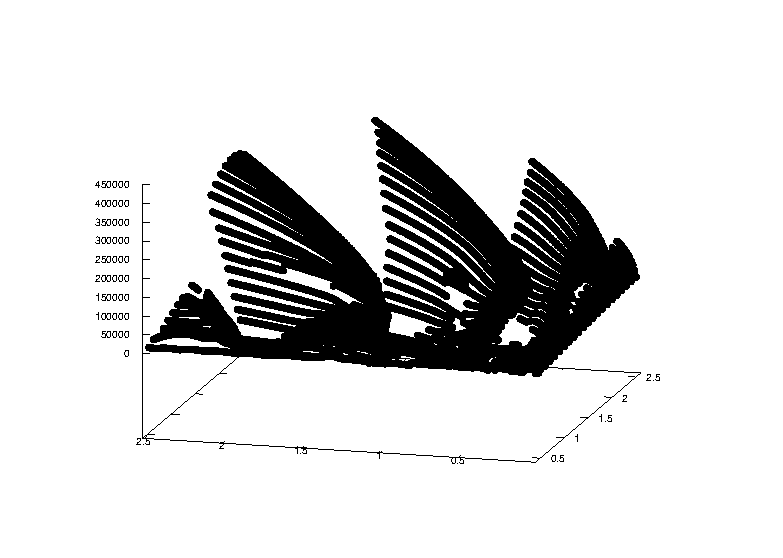
\includegraphics[width=\linewidth,angle=0]{pictures/gnuplot/3d/Hoehe/production/HoeheKraft.eps}
%	\end{center}	
%\end{figure}

\newpage

\subsection{Variation des Seitenverhältnisses}

Die Variation des Seitenverhältnisses wurde unter konstanter Fläche untersucht. Für eine gegebene Fläche $f$ und ein Seitenverhältnis $Sv$ können $a$ und $b$ wie folgt berechnet werden:

$$b = \left(\dfrac{f}{Sv}\right)^\frac{1}{2}$$
$$a = \dfrac{f}{b} $$

In Abbildung~\ref{fig:svMR} bildet sich eine klare Abhängigkeit der Stoßanzahl von dem Seitenverhältnis aus. Da mit einem steigendem Seitenverhältnis unter gleicher Fläche, eine der beiden Seitenlänge minimiert wird, dominiert diese Seite die Steifigkeit der Platte. Somit steigt das benötigte Massenverhältnis mit dem Seitenverhältnis, um mehr als einen Schlag zu erzielen. Ebenfalls steigt die Anzahl der Schläge mit steigenden Massenverhältnis. Jedoch hat das Massenverhältnis $MR$ einen deutlich kleineren Einfluss als das Seitenverhältnis.\\

\begin{figure}[H]
	\begin{center}
		\begin{overpic}[width=\linewidth]{pictures/gnuplot/3d/svMR/production/svmr.eps}
			\put(47,4){$a/b$ [-]}
			\put(73,64){Aufschläge [-]}
			\put(18,32){\rotatebox{90}{MR [-]}}
		\end{overpic}
		\caption{Anzahl der Aufschläge in Abhängigkeit des Seitenverhältnis}
		\label{fig:svMR}
	\end{center}
\end{figure}

Auffallend ist zudem noch das schnelle Ansteigen der Anzahl der Schläge bei einem Seitenverhältnis zwischen eins und ein-einhalb. Über diesem Intervall fällt die Anzahl der Schläge wieder. Wichtig zu erwähnen ist eine numerische Instabilität des Skriptes, welche bei z.B. hohen Massenverhältnissen zu weit überhöhten Durchbiegungen führt. Diesem Fall kann mit einer verringerten Schrittweite teilweise entgegengewirkt werden. Diese numerische Instabilität wird insbesondere ersichtlich, wenn die maximale Durchbiegung aufgetragen wird, siehe Abbildung~\ref{fig:svMRDurchbiegung}.

Hier fallen sehr hohe Durchbiegungen auf. Da die Vernachlässigung von Membrankräften in der Platte nur für kleine Durchbiegungen gültig ist, wird die tatsächliche Durchbiegung deutlich geringer sein.
Für die maximale Auslenkung sowie für die maximale Kraft ergibt sich ein ähnliches Bild, siehe Abbildung~\ref{fig:svmrKraft}. Mit steigender Impaktormasse steigen die Kraft und die Durchbiegung. Auffallend ist die eine maximale Durchbiegung für ein Seitenverhältnis von $2.2$. Dies ist insbesondere unerwartet, da die Steifigkeit der Platte für das gegebene Seitenverhältnis deutlich größer ist, als für den quadratischen Fall. Es ergibt sich ebenfalls eine maximale Kraft für das soeben genannte Seitenverhältnis von $2.2$. \\
Ab einem Seitenverhältnis $ Sv \geq 3.5$ sind die Durchbiegung und die maximale Kraft homogen und weisen keine Abhängigkeit von der Masse mehr auf.

\begin{figure}[H]
	\begin{center}
		\begin{overpic}[width=\linewidth]{pictures/gnuplot/3d/svmr/production/svmrAuslenkung.eps}
			\put(47,4){$a/b$ [-]}
			\put(73,64){Auslenkung [cm]}
			\put(18,32){\rotatebox{90}{$MR$ [-]}}
		\end{overpic}
		\caption{Maximale Durchbiegung in Abhängigkeit des Seitenverhältnis}
		\label{fig:svMRDurchbiegung}
	\end{center}
\end{figure}

\begin{figure}[H]
	\begin{center}
		\begin{overpic}[width=\linewidth]{pictures/gnuplot/3d/svMR/production/svmrKraftFixed.eps}
			\put(47,4){$a/b$ [-]}
			\put(73,64){Kraft [N]}
			\put(18,32){\rotatebox{90}{$MR$ [-]}}
		\end{overpic}
		\caption{Maximale Kraft in Abhängigkeit des Seitenverhältnis}
		\label{fig:svmrKraft}
	\end{center}
\end{figure}






	%Im zweiten Teil des Hauptteils folgt die Darstellung der eigenen Leistung. Aufbauend auf den im vorigen Kapitel erarbeiteten Grundlagen  wird nun der Lösungsweg aufgezeigt. Dabei wird das prinzipielle Vorgehen zum Erreichen der Zielsetzung unter Einbindung der verwendeten Hilfsmittel (Maschinen, Geräte, Programme etc. inklusive der verwendeten Einstellungen) aufgezeigt. Dabei müssen sämtliche verwendeten Daten ersichtlich sein, sodass es jederzeit möglich ist, die ermittelten Ergebnisse zu reproduzieren. Zum Schluss erfolgt unter Berücksichtigung der Randbedingungen eine kritische Analyse der Ergebnisse mit möglichen Unsicherheiten und Fehlern. Aus der Diskussion der Ergebnisse (z.B. Vergleich von Messwerten und theoretischen Vorhersagen), wird schließlich der Nutzen erörtert und mögliche weiterführende Fragestellungen werden erarbeitet.